\documentclass[t]{beamer}


\usepackage{header100}
\usepackage{header_maps}
\usepackage[utf8]{inputenc}


\usepackage{amsfonts}
\usepackage{amssymb}
\usepackage{amsmath}
\usepackage{times}
\usepackage{graphicx}
\usepackage{sidecap}
\usepackage{mathtools}
\usepackage{caption}
\usepackage{breakurl}
\usepackage{bm}
\usepackage[all]{xy}
\usepackage{lipsum}
\usepackage{amsthm}
\usepackage{tikz}
\usepackage{booktabs}
\usepackage{pgfplots}
\usepackage{tabularx}
\usetikzlibrary{positioning}
\usepackage{xurl}
\usepackage{animate}
\usetikzlibrary{shapes,snakes}

\pgfplotsset{compat=1.18}



\DeclarePairedDelimiter\ceil{\lceil}{\rceil}
\DeclarePairedDelimiter\floor{\lfloor}{\rfloor}

\DeclareMathOperator{\cok}{coker}
\DeclareMathOperator{\im}{im}
\DeclareMathOperator{\ann}{Ann}
\DeclareMathOperator{\Hom}{Hom}
\DeclareMathOperator{\vol}{vol}

\newcommand{\vv}{\vspace{0.3cm}}

\makeatletter
\newenvironment<>{proofs}[1][\proofname]{%
 \par
 \def\insertproofname{#1\@addpunct{.}}%
 \usebeamertemplate{proof begin}#2}
 {\usebeamertemplate{proof end}}
\makeatother

\newcommand{\ik}[1]{\begin{block}{iClicker Activity} #1 \end{block}}
\newcommand{\ex}[1]{\begin{block}{Exercise} #1 \end{block}}
\newcommand{\co}[1]{[#1)}
\newcommand{\oc}[1]{(#1]}
\newcommand{\p}{\pause}
\newcommand{\ddx}{\frac{d}{dx}}
\newcommand{\eb}[1]{\begin{exampleblock}{} #1 \end{exampleblock}}
\newcommand{\RR}{\mathbb{R}}
\newcommand{\ZZ}{\mathbb{Z}}

\newcommand{\KP}[1]{%
  \begin{tikzpicture}[baseline=-\dimexpr\fontdimen22\textfont2\relax]
  #1
  \end{tikzpicture}%
}
\newcommand{\KPA}{%
  \KP{\filldraw[color=gray, fill=none, thick] circle (0.3);}%
}

\newcommand{\KPUNLINK}{%
  \KP{\filldraw[color=gray, fill=none, thick] circle (0.3);
  \filldraw[color=gray, fill=none, thick] (0.7,0) circle (0.3);}%
}

\newcommand{\KPB}{%
  \KP{
 \draw[color=gray,thick] (-0.3,0.3) -- (0.3,-0.3);
 \draw[color=gray,thick] (-0.3,-0.3) -- (-0.05,-0.05);
 \draw[color=gray,thick] (0.05,0.05) -- (0.3,0.3);
  }%
}

\newcommand{\KPBB}{%
  \KP{
 \draw[color=gray,thick] (-0.3,-0.3) -- (0.3,0.3);
 \draw[color=gray,thick] (-0.3,0.3) -- (-0.05,0.05);
 \draw[color=gray,thick] (0.05,-0.05) -- (0.3,-0.3);
  }%
}

\newcommand{\KPC}{%
  \KP{%
 \draw[color=gray,thick] (-0.3,0.3) .. controls (0,-0.05) .. (0.3,0.3);
 \draw[color=gray,thick] (-0.3,-0.3) .. controls (0,0.05) .. (0.3,-0.3);
  }%
}
\newcommand{\KPD}{%
  \KP{%
 \draw[color=gray,thick] (-0.3,-0.3) .. controls (0.05,0) .. (-0.3,0.3);
 \draw[color=gray,thick] (0.3,-0.3) .. controls (-0.05,0) .. (0.3,0.3);
  }%
}

\newcommand{\tabitem}{%
  \usebeamertemplate{itemize item}\hspace*{\labelsep}}

\newcommand{\knotlinewidth}{.7pt}
\newcommand{\myarrow}{$\quad\longleftrightarrow\quad$}
\newcommand{\RIa}[1][]{\tikz[knot, #1]{\draw(-.5,.5) to[out=-90,in=-90] (.5,0); \draw[overcross] (.5,0) to[out=90,in=90] (-.5,-.5);}}
\newcommand{\RIb}[1][]{\tikz[knot, #1]{\draw[looseness=.8] (-.5,-.5) to[out=90, in=-90] (.5,0) to[out=90, in=-90] (-.5,.5);}}
\newcommand{\RIIa}[1][]{\tikz[knot, #1]{\draw[red, looseness=2.3] (-.5,-.5) to[out=0, in=0] (-.5,.5); \draw[looseness=2.3, overcross=blue] (.5,-.5) to[out=180, in=180] (.5,.5);}}
\newcommand{\RIIb}[1][]{\tikz[knot, #1]{\draw[red, looseness=1.4] (-.5,-.5) to[out=0, in=0] (-.5,.5);\draw[blue, looseness=1.4] (.5,.5) to[out=180,in=180] (.5,-.5);}}
\newcommand{\RIIc}[1][]{\tikz[knot, #1]{\draw[blue, looseness=2.3] (.5,-.5) to[out=180, in=180] (.5,.5); \draw[looseness=2.3, overcross=red] (-.5,-.5) to[out=0,in=0] (-.5,.5);}}
\newcommand{\RIIIa}[1][]{\tikz[knot, #1]{\draw[red] (-120:.58) to[out=60,in=-120] (150:.2) to[out=60, in=-120] (60:.58); \draw[rotate=-120, overcross=blue] (-120:.58) to[out=60, in=-120] (150:.2) to[out=60, in=-120] (60:.58); \draw[rotate=120, overcross=green!80!black] (-120:.58) to[out=60, in=-120] (150:.2) to[out=60, in=-120] (60:.58);}}


\tikzset{overcross/.style={double, line width=1.5, white, double=#1, double distance=\knotlinewidth},
 overcross/.default={black},
 knot/.style={line width=\knotlinewidth, baseline=-.5ex}}

%Information to be included in the title page:
\title{A Layman's Introduction to Knots and Jones Polynomials}
\institute{University of Manitoba}
\author{Junyu Lu}
\date{Nov 2023}
\titlegraphic{
\includegraphics[height=1cm]{pic/um.png}}

\begin{document}

\frame{\titlepage}

\begin{frame}[t]
	\frametitle{Definitions}
	\begin{center}
		Knot = A piece-wise linear (or smooth) embedding of $S^1$ into $\RR^3$ or $S^3$\\
		\vspace{0.1in}
		Link = A p.l. (or smooth) embedding of disjoint circles into $\RR^3$ or $S^3$
	\end{center}
	\p
	\begin{figure}
		\centering
		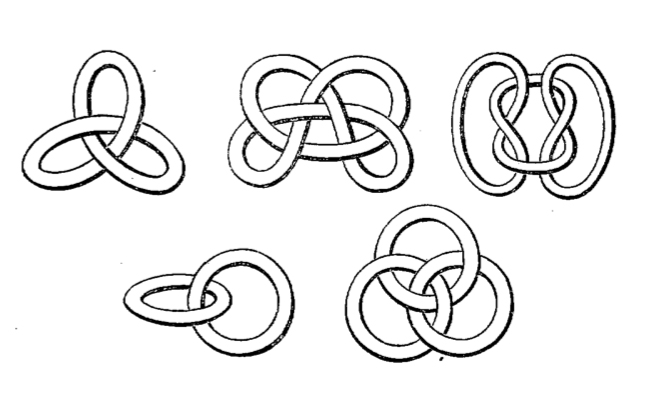
\includegraphics[width=6cm]{pic/kelvin_knots.jpg}
		\caption{Illustrations of knots and links, including a trefoil knot, top left, in an 1869 paper by Lord Kelvin on his knotted vortex theory of atoms.}
	\end{figure}
\end{frame}


\begin{frame}[t]
	\frametitle{Definitions}
	\begin{center}
		Knot = A piece-wise linear (or smooth) embedding of $S^1$ into $\RR^3$ or $S^3$\\
		\vspace{0.1in}
		Link = A p.l. (or smooth) embedding of disjoint circles into $\RR^3$ or $S^3$
	\end{center}

	\begin{figure}
		\centering
		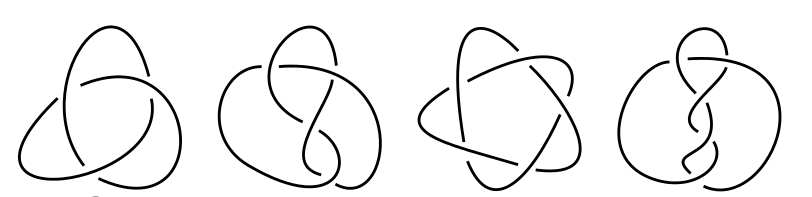
\includegraphics[width=10cm]{pic/prime-knots.png}
	\end{figure}

	\begin{block}{Knot Diagrams}
		A picture of a projection of a knot onto a plane
	\end{block}
\end{frame}

\begin{frame}[c]
	\frametitle{Knot Equivalence}
	Two knots are \emph{equivalent} if one knot can be pushed about smoothly, without intersecting itself, to coincide with another knot.

	\begin{figure}
		\centering
		\animategraphics[loop,controls,width=3.5cm]{10}{pic/Knot_Unfolding-}{0}{50}
		\caption{Deformation to an unknot}
	\end{figure}
	\vspace{-0.4cm}
	\begin{center}
		unknot = the boundary of a simplicial disk
	\end{center}

	%Or more rigorously, defined by ambient isotopy or equivalently by an orientation-preserving homeomorphism of $S^3$ to itself

\end{frame}

\begin{frame}
	\frametitle{Reidemeister Moves}
	\begin{theorem}[Reidemeister 1927]
		Two knots are equivalent if and only if all their diagrams are connected by a finite sequence of Reidemeister moves of Type I, II or III.
	\end{theorem}
	\begin{center}
		\begin{minipage}{0.5\textwidth}
			\begin{enumerate}[I.]
				\item \RIa\myarrow\RIb
				\item \RIIa\myarrow\RIIb
				\item \RIIIa\myarrow\RIIIa[rotate=180]
			\end{enumerate}
		\end{minipage}
	\end{center}

	In this case, we also say their diagrams are equivalent.
\end{frame}

\begin{frame}
	\frametitle{Reidemeister Moves}

	\begin{block}{Remark}
		The following moves can be seen (exercise) to be consequences of the three types of Reidemeister moves.
	\end{block}
	\begin{center}
		\begin{minipage}{0.5\textwidth}
			\begin{enumerate}[I.']
				\item \RIa[yscale=-1]\myarrow\RIb
				\item \RIIc\myarrow\RIIb
				\item \RIIIa[xscale=-1]\myarrow\RIIIa[xscale=-1, rotate=180]
			\end{enumerate}
		\end{minipage}
	\end{center}
\end{frame}

\begin{frame}
	\frametitle{Reidemeister Moves}
	\begin{center}
		\begin{minipage}{0.5\textwidth}
			\begin{enumerate}[I.]
				\item \RIa\myarrow\RIb
				\item \RIIa\myarrow\RIIb
				\item \RIIIa\myarrow\RIIIa[rotate=180]
			\end{enumerate}
		\end{minipage}
	\end{center}

	\vspace{0.4cm}

	\begin{figure}
		\centering
		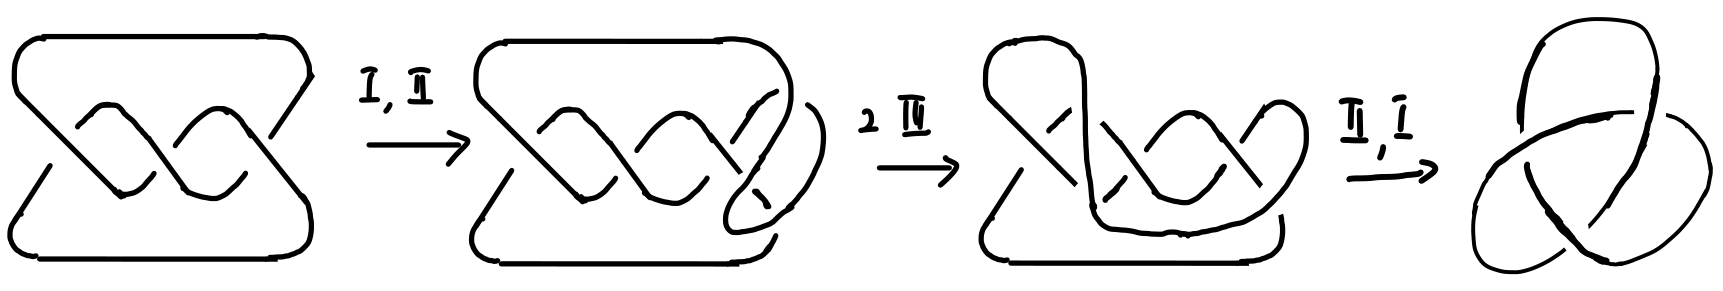
\includegraphics[width=10.5cm]{pic/rmseq.png}
	\end{figure}
\end{frame}


\begin{frame}[c]
	\begin{block}{Recognition Problem}
		Given two knots/knot diagrams, determining the (non-)equivalence of two knots.
	\end{block}

	\begin{block}{Unkotting Problem}
		Given a knot (diagram), determining whether it is the unknot.
	\end{block}
	\p
	{\small{\begin{itemize}
				\item Both problems are NP.
				\item $n=$ the sum of crossing numbers of two diagrams; an upper bound on the number of Reidemeister moves is $2^{2^{2^{\dots^n}}}$, where where the height of the tower of $2$s is $10^{1,000,000n}$ (Coward \& Lackenby 2014).
				\item $c=$ the sum of crossing numbers of an unknot diagram; an upper bound on the number of Reidemeister moves required to arrive at the standard unknot is $(236c)^{11}$ (Lackenby 2015).
			\end{itemize}}}
\end{frame}

\begin{frame}[c]
	\frametitle{Unknotting Problem}
	\begin{figure}[!htb]
		\centering
		\begin{minipage}{5cm}
			\centering
			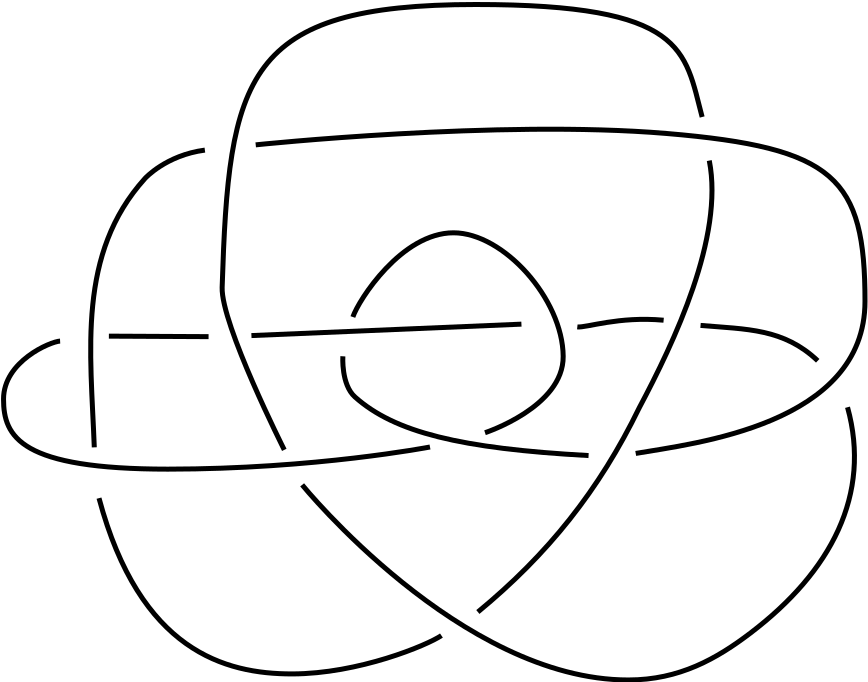
\includegraphics[width=4cm]{pic/Ochiai_unknot.png}
			\caption{One of Ochiai's unknots}
		\end{minipage}
		\begin{minipage}{4.4cm}
			\centering
			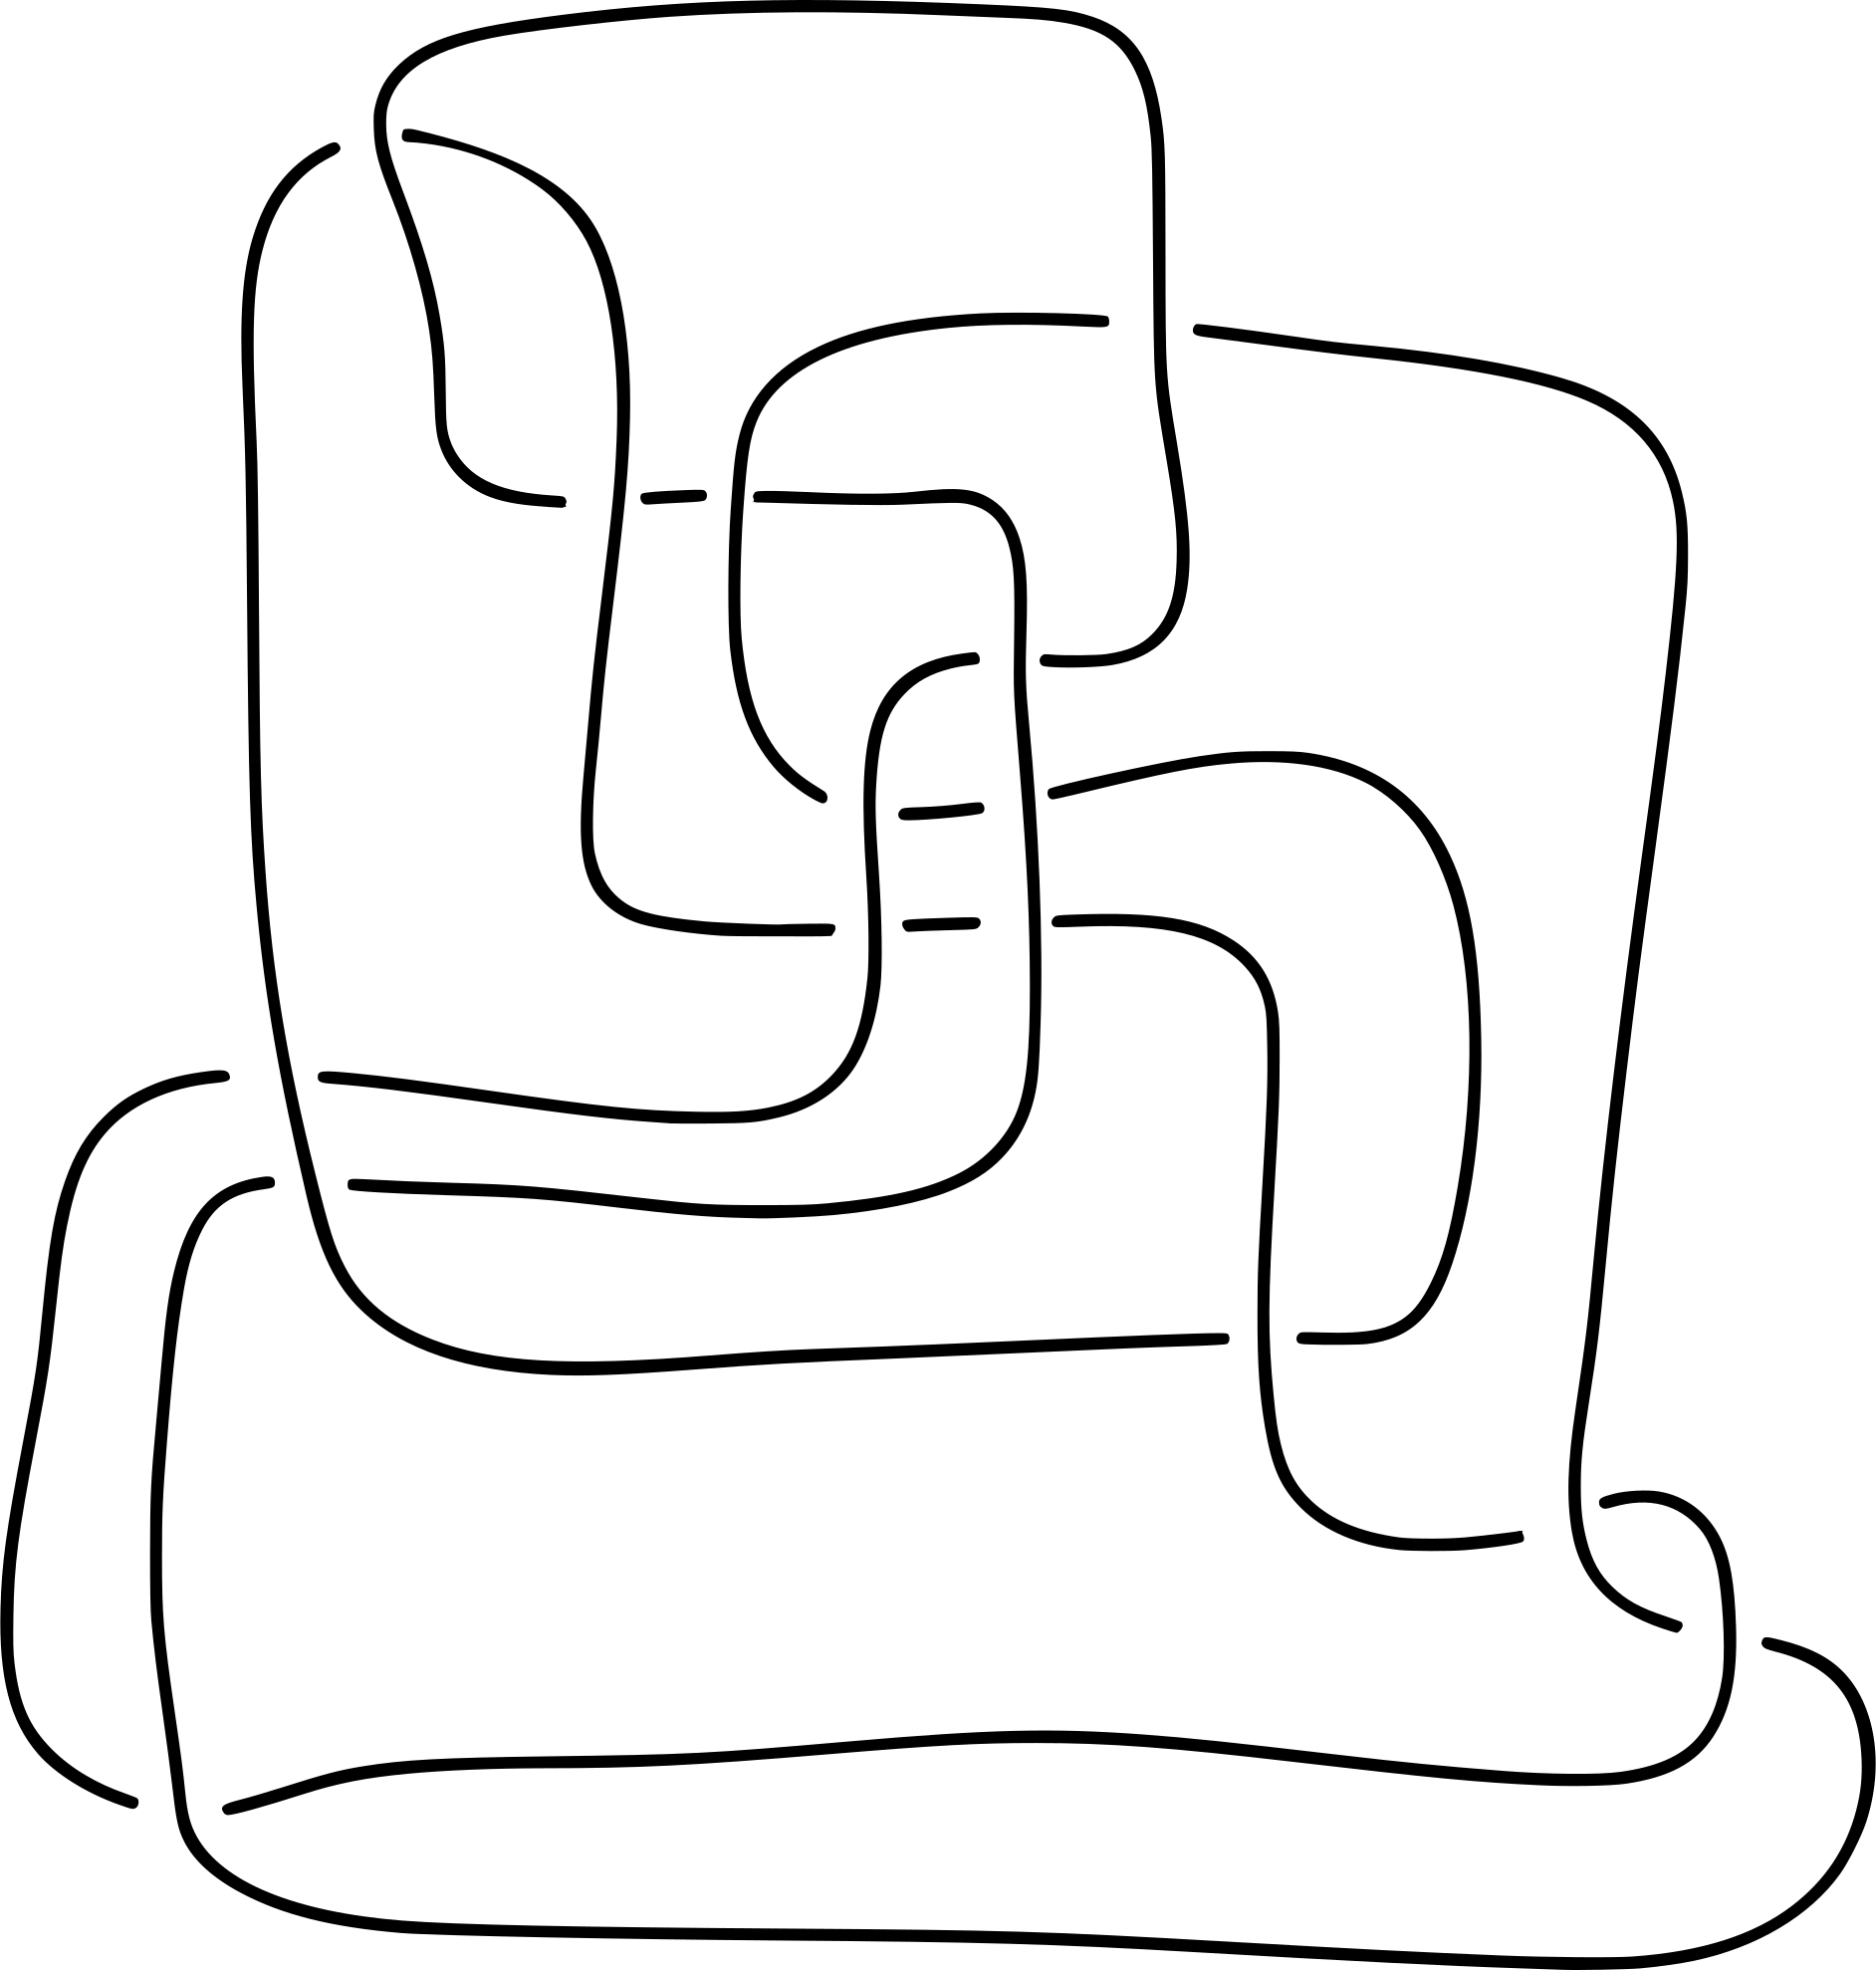
\includegraphics[width=3cm]{pic/Thistlethwaite_unknot.png}
			\caption{Thistlethwaite unknot}
		\end{minipage}
	\end{figure}

	Not easy, actually very hard, to see both of the knots above are the unknot.

\end{frame}

\begin{frame}[c]
	\frametitle{Knot Complements}
	\begin{tabular}{ l l }
		{Knot:}                  & $K \subset S^3$       \\
		{Regular neighbourhood:} & $n(K)$                \\
		{Knot complement:}       & $\overline{S^3-n(K)}$
	\end{tabular}
	\vspace{0.3cm}
	\[K_1=K_2 \quad\Longrightarrow\quad \overline{S^3-n(K_1)}=\overline{S^3-n(K_2)} \]

	\begin{center}
		Invariants of $\overline{S^3-n(K)}\quad \Longrightarrow \quad$ Invariants of $K$
	\end{center}

	\begin{block}{Topological and Geometric Invariants}
		\begin{itemize}
			\item $\pi_1(K)=\pi_1(\overline{S^3-n(K)})$, the knot group of $K$
			\item Hyperbolic volume of $\overline{S^3-n(K)}=\vol(K)$, the volume of $K$
		\end{itemize}
	\end{block}
	\p
	\vspace{0.2cm}
	Fact: The only knot with infinite cyclic knot group is the unknot.

\end{frame}

% \begin{frame}
% 	\frametitle{Knot Complements}
% 	\small
% 	\begin{theorem}[Gordon and Luecke 1989]
% 		If $K_1$ and $K_2$ are unoriented knots in $S^3$ and there is an orientation preserving homeomorphism between their complements, then $K_1$ and $K_2$ are equivalent (as unoriented knots).
% 	\end{theorem}

% 	\begin{theorem}[Whitten 1987]
% 		If $K_1$ and $K_2$ are prime knots in $S^3$ with isomorphic knot groups, then their complements are homeomorphic.
% 	\end{theorem}

% 	\begin{theorem}[Waldhausen 1966]
% 		If there exists an isomorphism between two knot groups sending longitude to longitude and meridian to meridian, then these two knots are equivalent.
% 	\end{theorem}

% \end{frame}

\begin{frame}[c]
	\frametitle{Diagrammatic Invariant}
	\begin{block}{Idea}
		\begin{center}
			Knots are equivalent $\Longleftrightarrow$ Knot diagrams are equivalent\\
			\vspace{0.1cm}
			Diagrammatic invariants: invariants that respect Reidemeister moves
		\end{center}
	\end{block}
	\p
	A diagrammatic polynomial invariant:
	\begin{tabular}{ l l }
		{Knot:}            & $K \subset S^3$                     \\
		{Knot polynomial:} & $f(K)\in \ZZ[t]$ or $\ZZ[t,t^{-1}]$ \\
		                   & $f(\RIa ) = f(\RIb)$                \\
		                   & $f(\RIIa ) = f(\RIIb)$              \\
		                   & $f(\RIIIa) = f(\RIIIa[rotate=180])$
	\end{tabular}
\end{frame}

\begin{frame}
	\frametitle{Kauffman Bracket}
	\begin{definition}
		The Kauffman bracket is a function from unoriented link diagrams in the oriented plane to Laurent polynomials $\ZZ[A,A^{-1}]$. It maps a diagram $D$ to $\left\langle D\right\rangle \in\ZZ[A,A^{-1}]$ and is
		characterized by
		\begin{enumerate}
			\item[1.] $\left\langle\KPA\right\rangle=1$;
			\item[2.] $\left\langle L \cup \KPA\right\rangle=(-A^{2}-A^{-2})\langle L\rangle$;
			\item[3.] $\left\langle\KPB\right\rangle= A\left\langle\KPC\right\rangle + A^{-1} \left\langle \KPD \right\rangle$.
		\end{enumerate}
		Or if you tilt your head $\frac{\pi}{2}$,
		\begin{enumerate}
			\item[3'.] $\left\langle\KPBB\right\rangle= A\left\langle\KPD\right\rangle + A^{-1} \left\langle \KPC \right\rangle$.
		\end{enumerate}
	\end{definition}
\end{frame}

\begin{frame}
	\frametitle{Kauffman Bracket}
	\begin{block}{Observation}
		Given a knot diagram, if you change all $\KPB$ to either $\KPC$ or $\KPD$, then you arrive at an unlink.
	\end{block}

	\begin{enumerate}
		\item[1.] $\left\langle\KPA\right\rangle=1$;
		\item[2.] $\left\langle L \cup \KPA\right\rangle=(-A^{2}-A^{-2})\langle L\rangle$;
		\item[3.] $\left\langle\KPB\right\rangle= A\left\langle\KPC\right\rangle + A^{-1} \left\langle \KPD \right\rangle$.
	\end{enumerate}
	% Or if you tilt your head $\frac{\pi}{2}$,
	% \begin{enumerate}
	% 	\item[3'.] $\left\langle\KPBB\right\rangle= A\left\langle\KPD\right\rangle + A^{-1} \left\langle \KPC \right\rangle$.
	% \end{enumerate}
	\vspace{0.4cm}

	Applying this rules repetitively, we get a Laurent polynomial.

\end{frame}

\begin{frame}
	\frametitle{Kauffman Bracket}
	\begin{enumerate}
		\item[1.] $\left\langle\KPA\right\rangle=1$;
		\item[2.] $\left\langle L \cup \KPA\right\rangle=(-A^{2}-A^{-2})\langle L\rangle$;
		\item[3.] $\left\langle\KPB\right\rangle= A\left\langle\KPC\right\rangle + A^{-1} \left\langle \KPD \right\rangle$.
	\end{enumerate}

	\vspace{0.2cm}
	An easy calculation with the unlink:
	\begin{align*}
		\left\langle\KPUNLINK\right\rangle & = (-A^{2}-A^{-2})\left\langle\KPA\right\rangle \\
		                                   & =-A^2-A^{-2}
	\end{align*}


\end{frame}

\begin{frame}
	\frametitle{Kauffman Bracket}
	\begin{enumerate}
		\item[1.] $\left\langle\KPA\right\rangle=1$;
		\item[2.] $\left\langle L \cup \KPA\right\rangle=(-A^{2}-A^{-2})\langle L\rangle$;
		\item[3.] $\left\langle\KPB\right\rangle= A\left\langle\KPC\right\rangle + A^{-1} \left\langle \KPD \right\rangle$.
	\end{enumerate}
	\vspace{0.4cm}
	Recall that
	\[\left\langle\KPUNLINK\right\rangle   =-A^2-A^{-2}. \]
	Another example:
	\begin{align*}
		\left\langle \raisebox{-10pt}{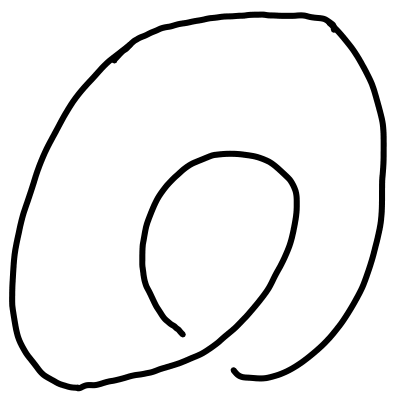
\includegraphics[width=1cm]{pic/kbun1.png}} \right\rangle & = A   \left\langle \raisebox{-10pt}{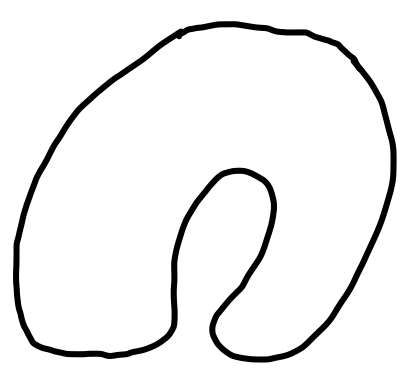
\includegraphics[width=1cm]{pic/kbun2.png}} \right\rangle  + A^{-1}\left\langle \raisebox{-10pt}{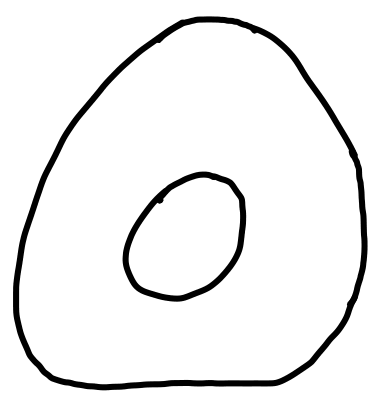
\includegraphics[width=1cm]{pic/kbun3.png}} \right\rangle \\
		                                                                                        & =A\cdot 1 + A^{-1}(-A^2-A^{-2})                                                                                                                                                                \\
		                                                                                        & = -A^{-3}
	\end{align*}

\end{frame}

\begin{frame}
	\frametitle{Kauffman Bracket}
	\vspace{-0.4cm}
	\begin{align*}
		\left\langle \raisebox{-10pt}{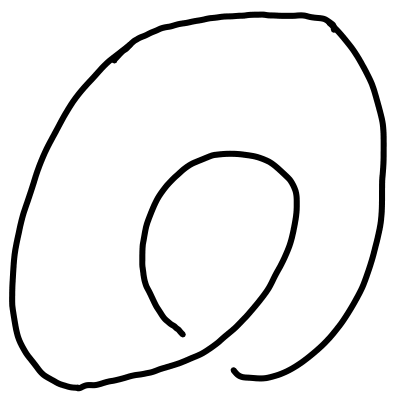
\includegraphics[width=1cm]{pic/kbun1.png}} \right\rangle & = A   \left\langle \raisebox{-10pt}{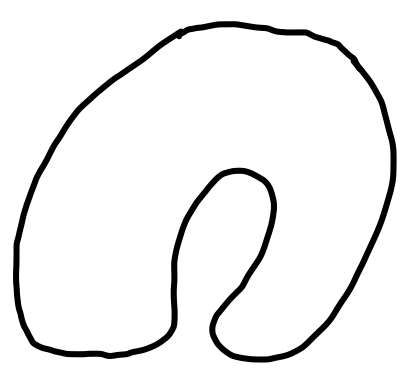
\includegraphics[width=1cm]{pic/kbun2.png}} \right\rangle  + A^{-1}\left\langle \raisebox{-10pt}{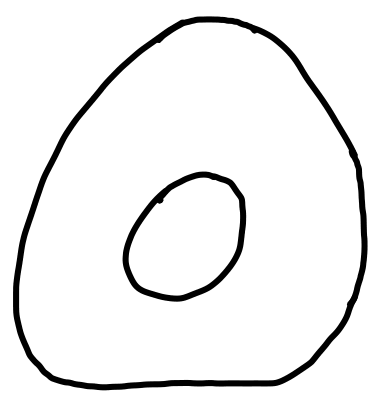
\includegraphics[width=1cm]{pic/kbun3.png}} \right\rangle \\
		                                                                                        & =A\cdot 1 + A^{-1}(-A^2-A^{-2})                                                                                                                                                                \\
		                                                                                        & = -A^{-3}
	\end{align*}
	\vspace{-0.4cm}
	\begin{block}{Good News}
		The Kauffman bracket respects Reidemeister moves of Type II and III.
	\end{block}

	\begin{block}{Bad News}
		The Kauffman bracket does \alert{not} respect Reidemeister moves of Type I.
	\end{block}
	Indeed, Type I gives an extra $-A^3$ factor and Type I' $-A^{-3}$.
	% {\small
	% \hspace*{-1cm}
	% \begin{tabular}{ l l }
	% 	Bad news:  & The Kauffman bracket does \emph{not} respect Reidemeister moves of Type I. \\
	% 	Good news: & The Kauffman bracket respects Reidemeister moves of Type II and III.
	% \end{tabular}
	% }

\end{frame}

\begin{frame}
	\frametitle{Writhe}
	\begin{block}{Oriented Link}
		A link with a choice of orientation for each complement
	\end{block}
	\begin{Definition}
		The writhe $w(D)$ of a diagram $D$ of an \emph{oriented} link is the sum of signs of the crossings of $D$, where each crossing has sign $+1$ or $-1$ according to the following:
	\end{Definition}

	\begin{center}
		\begin{tabular}{ c c }
			+1:\raisebox{-10pt}{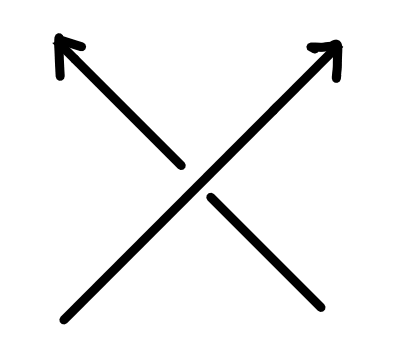
\includegraphics[width=1.5cm]{pic/lplus.png}} &
			-1: \raisebox{-10pt}{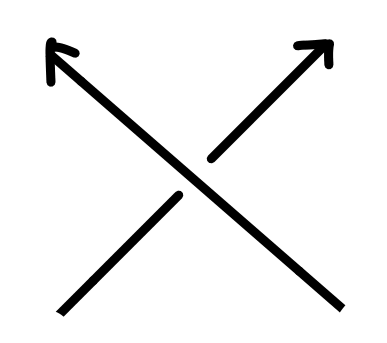
\includegraphics[width=1.5cm]{pic/lmin.png}}
		\end{tabular}
	\end{center}

\end{frame}


\begin{frame}[c]
	\frametitle{}

	\begin{block}{Property of Writhe}
		\begin{itemize}
			\item $w(D)$ does not change if $D$ is changed under Reidemeister moves of Type II or III.
			\item $w(D)$ does change by $+1$ or $-1$ if $D$ is changed under a Reidemeister move of Type I.
			\item The writhe of a knot diagram does \emph{not} depend on the choice of orientation.
		\end{itemize}
	\end{block}

	\begin{align*}
		w(\raisebox{-15pt}{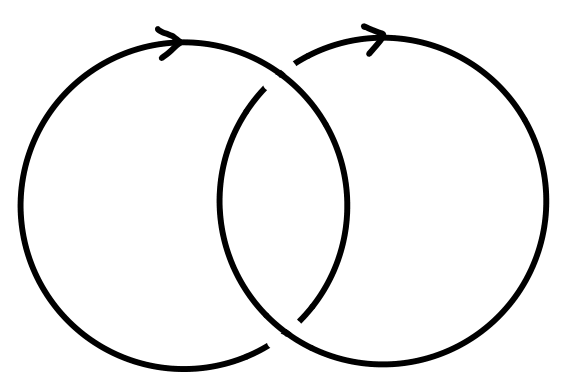
\includegraphics[width=1.8cm]{pic/holflp.png}})  = +2; \quad & w(\raisebox{-15pt}{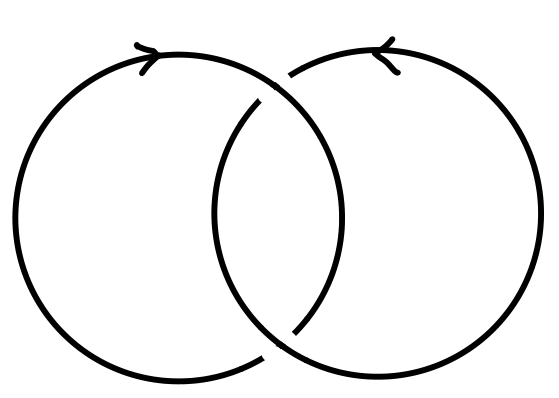
\includegraphics[width=1.8cm]{pic/holfpr.png}})=-2 \\
		w(\raisebox{-15pt}{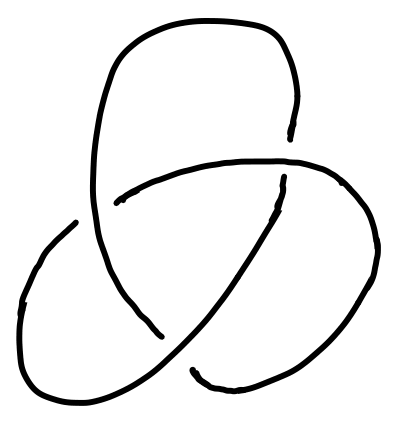
\includegraphics[width=1.4cm]{pic/trifoil.png}})             & =-3
	\end{align*}

\end{frame}

\begin{frame}[c]
	\frametitle{Jones Polynomial}
	\begin{theorem}
		Let $D$ be a diagram of an oriented link $L$. Then the expression \[(-A)^{-3w(D)}\langle D\rangle\] is an invariant of the oriented link $L$.
	\end{theorem}

	\begin{block}{Definition-Theorem}
		The Jones polynomial $V(L)$ of an oriented link $L$ is the Laurent polynomial in $t^{1/2}$ with integral coefficients, defined by \[V(L)= \left( (-A)^{-3w(D)}\langle D\rangle \right)_{t^{1/2}=A^{-2}} \in \ZZ[t^{1/2},t^{-1/2}],\] where $D$ is any oriented diagram for $L$.
	\end{block}
\end{frame}

\begin{frame}
	\frametitle{Hopf Link}
	\begin{align*}
		\left\langle \raisebox{-10pt}{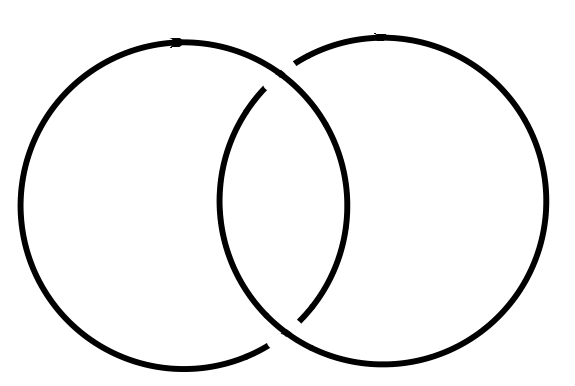
\includegraphics[width=1.6cm]{pic/hopf.png}} \right\rangle & = A\left\langle \raisebox{-10pt}{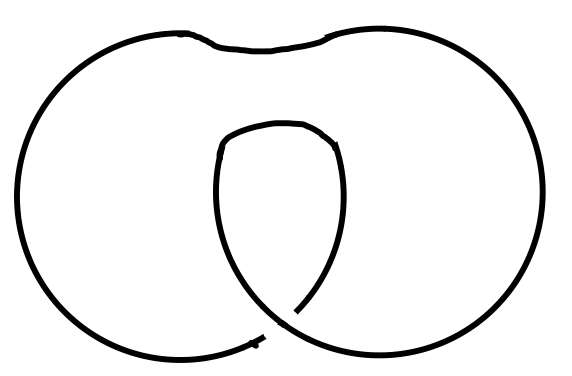
\includegraphics[width=1.6cm]{pic/hopfunkot2.png}} \right\rangle +A^{-1} \left\langle \raisebox{-10pt}{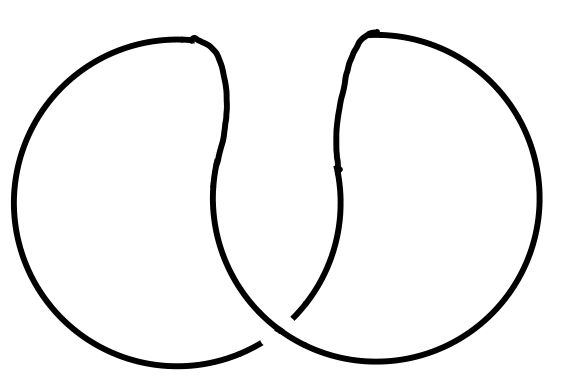
\includegraphics[width=1.6cm]{pic/hopfunkot1.png}} \right\rangle \\
		                                                                                         & = A(-A^3)+A^{-1} (-A^{-3}) =-A^4-A^{-4}                                                                                                                                                                  \\
		w(\raisebox{-10pt}{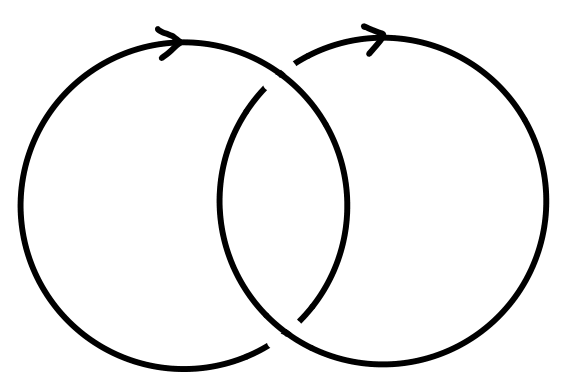
\includegraphics[width=1.6cm]{pic/holflp.png}})                       & =2;\quad w(\raisebox{-10pt}{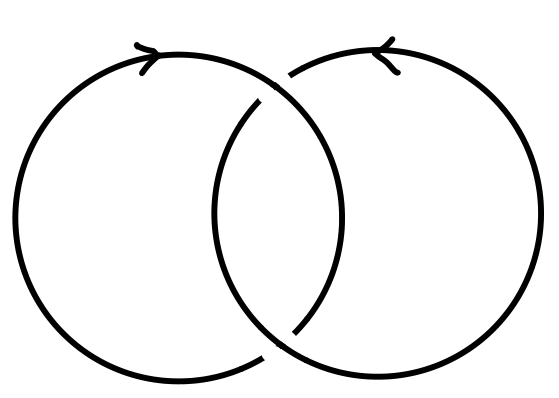
\includegraphics[width=1.6cm]{pic/holfpr.png}}) =-2
		                                                                                         &                                                                                                                                                                                                          \\
		V(\raisebox{-10pt}{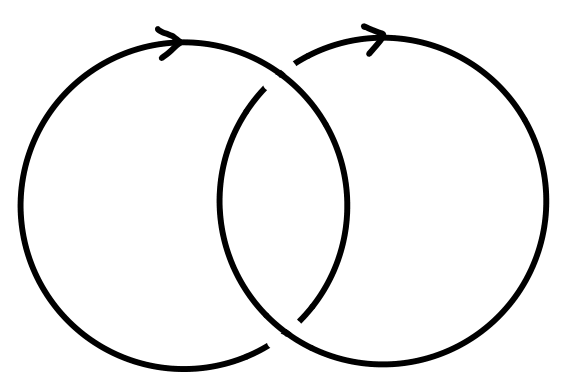
\includegraphics[width=1.6cm]{pic/holflp.png}})                       & = \left(-A^{-2}-A^{-10}\right)_{t^{1/2}=A^{-2}} = -t^{1/2}-t^{5/2}                                                                                                                                       \\
		V(\raisebox{-10pt}{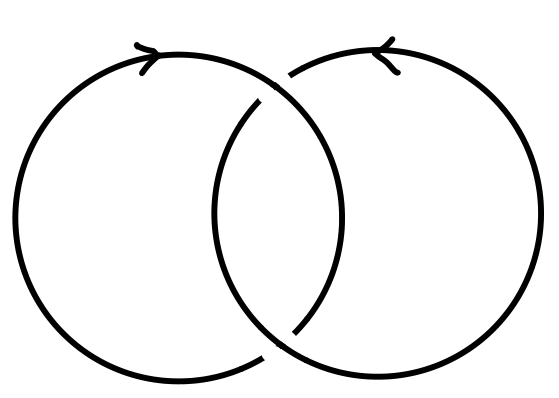
\includegraphics[width=1.6cm]{pic/holfpr.png}})                       & = \left(-A^{10}-A^{2}\right)_{t^{1/2}=A^{-2}} = -t^{-5/2}-t^{-1/2}
	\end{align*}

\end{frame}

\begin{frame}[c]
	\frametitle{Left-handed Trefoil Knot}

	\begin{align*}
		\left\langle \raisebox{-20pt}{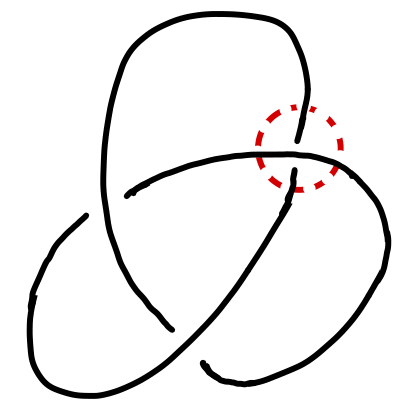
\includegraphics[width=1.8cm]{pic/trifoilkaff.png}} \right\rangle & = A\left\langle \raisebox{-20pt}{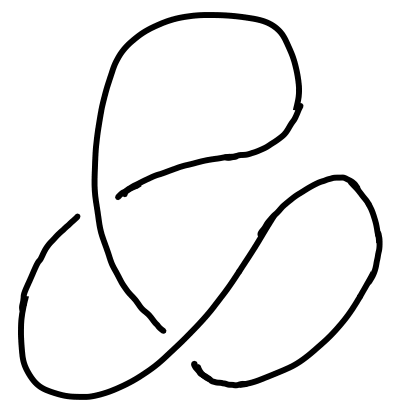
\includegraphics[width=1.8cm]{pic/trifoilkaff1.png}} \right\rangle +A^{-1} \left\langle \raisebox{-20pt}{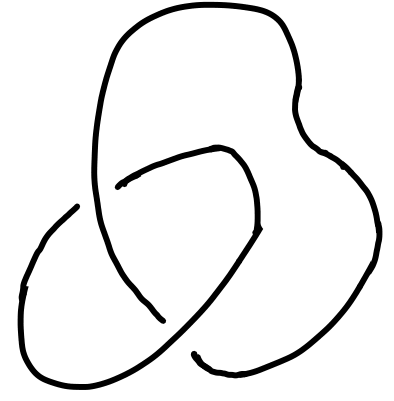
\includegraphics[width=1.8cm]{pic/trifoilkaff2.png}} \right\rangle \\
		                                                                                                & = A(-A^3)^2+A^{-1} (-A^{-4}-A^4) =A^7-A^3-A^{-5}                                                                                                                                                             \\
		w(\raisebox{-20pt}{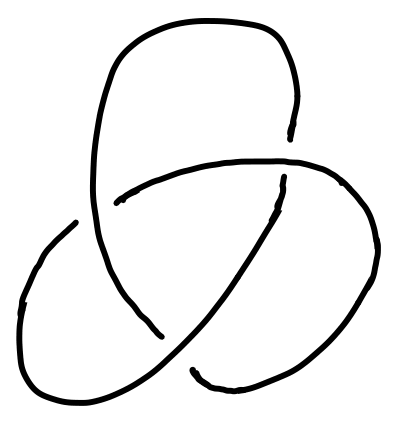
\includegraphics[width=1.8cm]{pic/trifoil.png}})                             & =-3                                                                                                                                                                                                          \\
		V(\raisebox{-20pt}{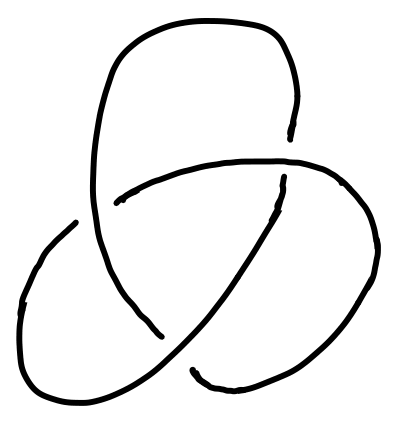
\includegraphics[width=1.8cm]{pic/trifoil.png}})                             & = \left(-A^{16}+A^{12}+A^4\right)_{t^{1/2}=A^{-2}} = -t^{-4}+t^{-3}+t^{-1}
	\end{align*}

\end{frame}

\begin{frame}[c]
	\frametitle{Right-handed Trefoil Knot}
	\begin{align*}
		\left\langle \raisebox{-20pt}{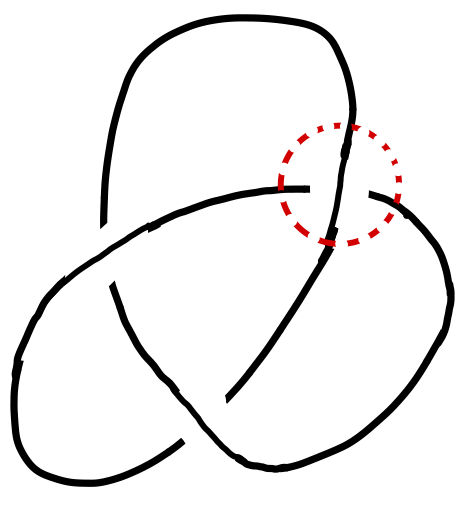
\includegraphics[width=1.8cm]{pic/trifoilrightkaff.png}} \right\rangle & = A\left\langle \raisebox{-20pt}{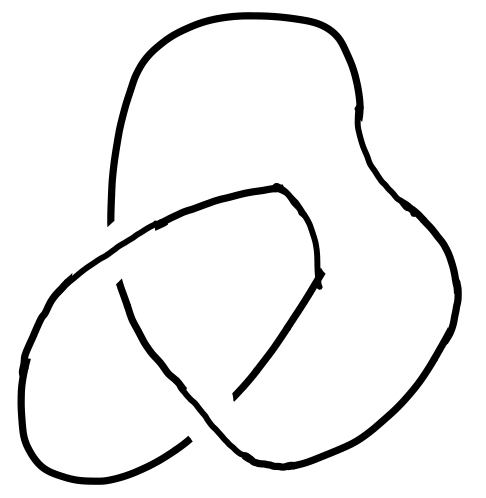
\includegraphics[width=1.8cm]{pic/trifoilrightkaff1.png}} \right\rangle +A^{-1} \left\langle \raisebox{-20pt}{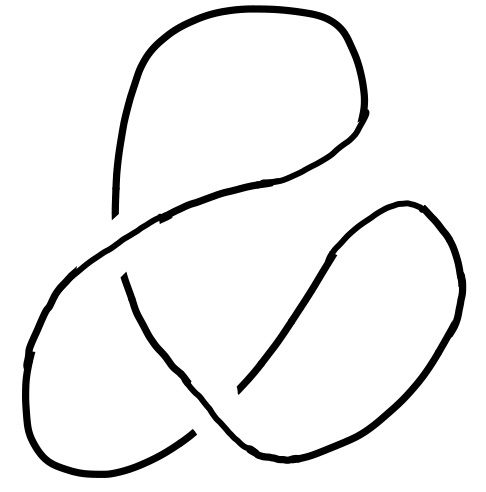
\includegraphics[width=1.8cm]{pic/trifoilrightkaff2.png}} \right\rangle \\
		                                                                                                     & = A(-A^4-A^{-4})+A^{-1} (-A^{-3})^2 =A^{-7}-A^{-3}-A^{5}                                                                                                                                                               \\
		w(\raisebox{-20pt}{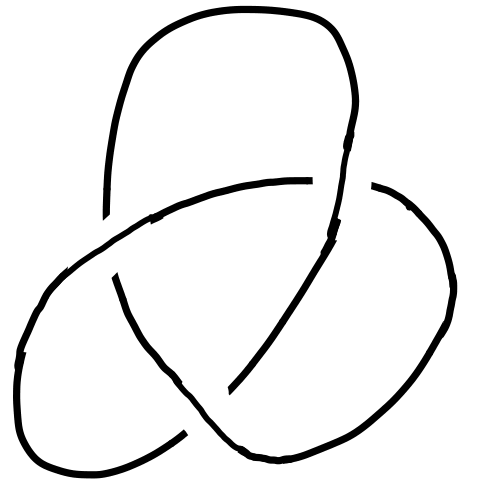
\includegraphics[width=1.8cm]{pic/righttrefoil.png}})                             & =3                                                                                                                                                                                                                     \\
		V(\raisebox{-20pt}{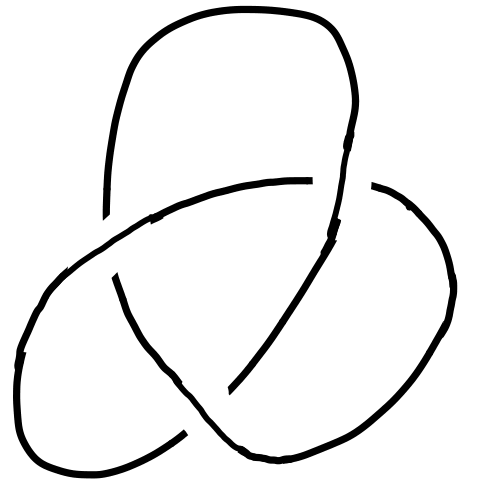
\includegraphics[width=1.8cm]{pic/righttrefoil.png}})                             & = \left(-A^{-16}+A^{-12}+A^{-4}\right)_{t^{1/2}=A^{-2}} = -t^{4}+t^{3}+t^{1}
	\end{align*}


\end{frame}

\begin{frame}
	\frametitle{Mirror Image}

	\begin{block}{Mirror Image}
		Put a mirror aside a knot and the image of the knot is known as the mirror image of the knot, or mathematically, the knot obtained by a refection in a plane.
	\end{block}
	\begin{figure}
		\centering
		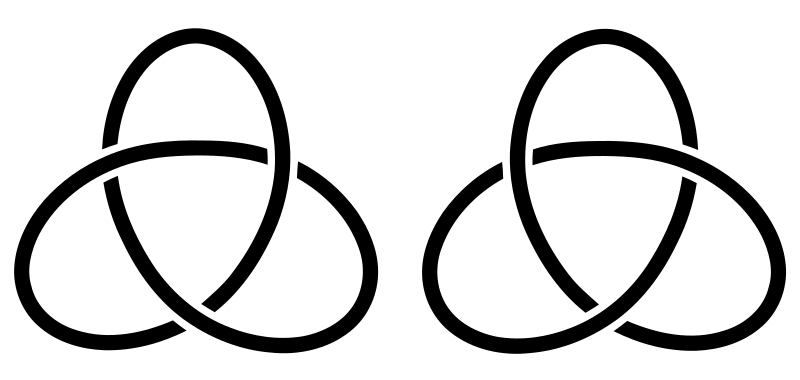
\includegraphics[width=6cm]{pic/The_two_trefoil_knots.png}
		\caption{The right-handed and left-handed trefoil knots are not equivalent}
	\end{figure}

\end{frame}

\begin{frame}
	\frametitle{Properties of Jones Polynomials}
	\begin{theorem}
		The Jones polynomial of the mirror image $\bar L$ of an oriented link $L$ is the conjugate under $t\leftrightarrow t^{-1}$ of the polynomial of $L$.
	\end{theorem}
	\p
	\begin{proofs}
		The mirror image negates the writhe of any oriented diagram by exchange the positive and negative crossings. The mirror effect on the Kauffman bracket is that $A$ is replaced by $A^{-1}$.
	\end{proofs}

	\begin{align*}
		V(\mbox{left-handed trefoil knot})  & = -t^{-4}+t^{-3}+t^{-1} \\
		V(\mbox{right-handed trefoil knot}) & = -t^{4}+t^{3}+t^{1}
	\end{align*}

\end{frame}

\begin{frame}[c]
	\frametitle{Connected Sum}

	% \begin{block}{Connected sum of knots}
	% 	To define the connected sum for two oriented knots:
	% 	\begin{itemize}
	% 		\item Consider a planar projection of each knot and suppose these projections are disjoint.
	% 		\item Find a rectangle in the plane where one pair of sides are arcs along each knot but is otherwise disjoint from the knots and so that the arcs of the knots on the sides of the rectangle are oriented around the boundary of the rectangle in the same direction.
	% 		\item Now join the two knots together by deleting these arcs from the knots and adding the arcs that form the other pair of sides of the rectangle.
	% 	\end{itemize}
	% \end{block}
	Connected sum of (oriented) knots $K_1\#K_2$:

	\begin{figure}
		\centering
		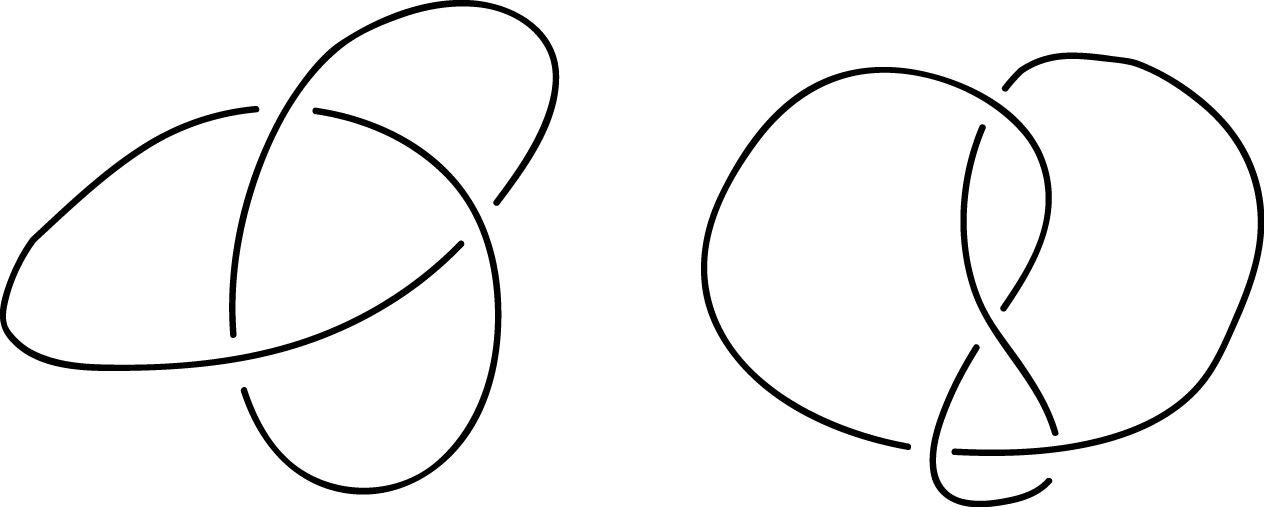
\includegraphics[width=4cm]{pic/Sum_of_knots.png}
		\vfill
		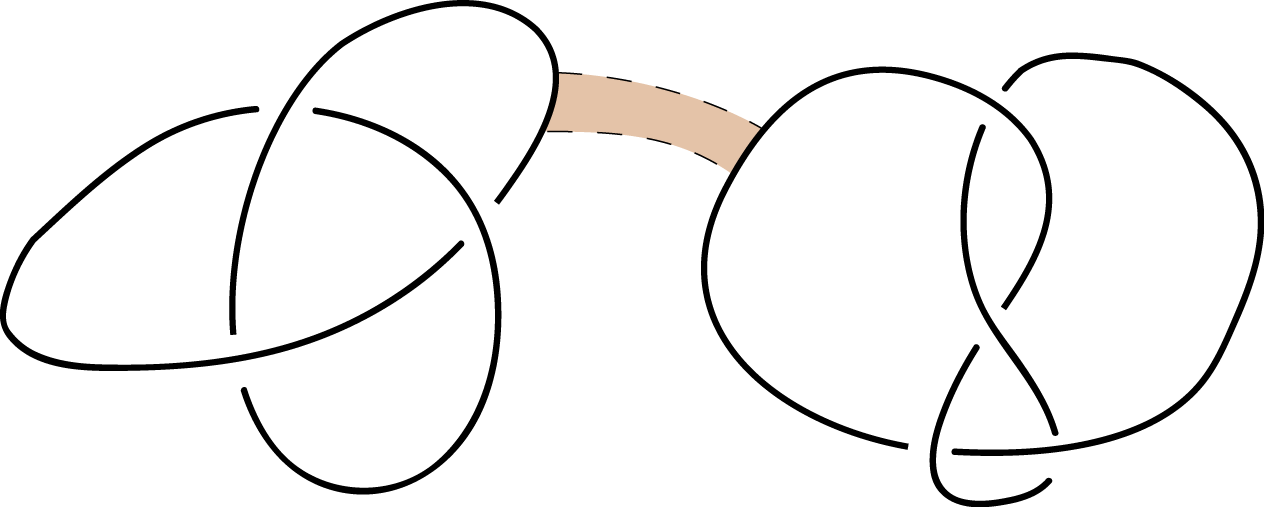
\includegraphics[width=4cm]{pic/Sum_of_knots2.png}
		\vfill
		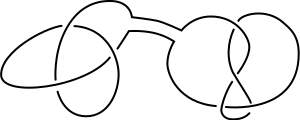
\includegraphics[width=4cm]{pic/Sum_of_knots3.png}
	\end{figure}
\end{frame}

\begin{frame}
	\frametitle{Properties of Jones Polynomials}
	\begin{theorem}
		Let $K_1, K_2$ be two (oriented) knots. Then we have \[V(K_1\# K_2)=V(K_1)V(K_2).\]
	\end{theorem}
	\begin{block}{Sketch of proof}
		Consider a calculation of the polynomial of $K_1\#K_2$ and operate firstly on the crossings of just one summand.
	\end{block}

	\begin{figure}
		\centering
		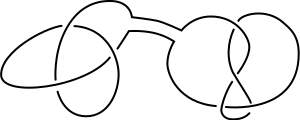
\includegraphics[width=4cm]{pic/Sum_of_knots3.png}
	\end{figure}

\end{frame}


\begin{frame}
	\frametitle{Yet Another Approach}

	\begin{block}{Definiton-Theorem}
		The Jones polynomial invariant is a function from the set of oriented links in $S^3$ to $\ZZ[t^{1/2},t^{-1/2}]$ such that \begin{enumerate}[I.]
			\item $V(\KPA)=1$;
			\item whenever three oriented links $L_+, L_-$ and $L_0$ are the same, except in the neighbourhood of a point where they are shown below, then
			      \[t^{-1}V(L_+)- tV(L_-)+(t^{-1/2}-t^{1/2})V(L_0)=0.\]
		\end{enumerate}
	\end{block}
	\begin{center}
		\begin{tabular}{ l  l l }
			$L_+$: \raisebox{-10pt}{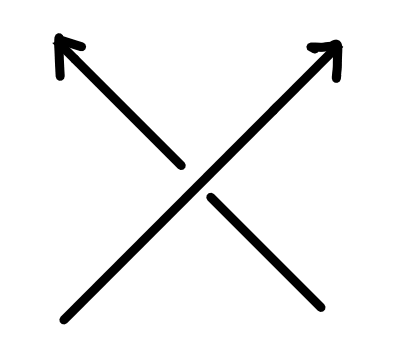
\includegraphics[width=1.5cm]{pic/lplus.png}} & $L_-$:\raisebox{-10pt}{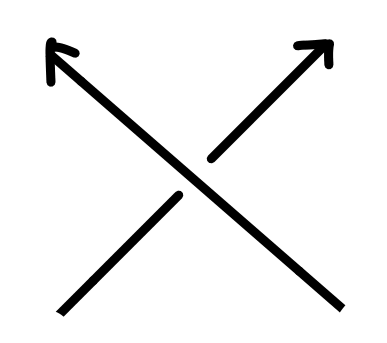
\includegraphics[width=1.5cm]{pic/lmin.png}} & $L_0$:\raisebox{-10pt}{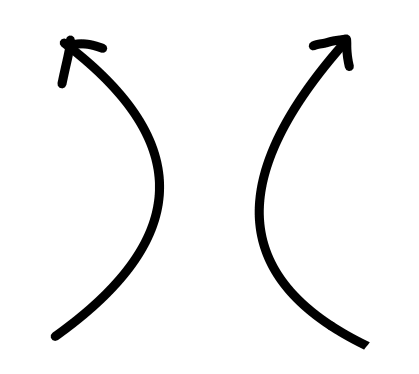
\includegraphics[width=1.5cm]{pic/l0.png}}
		\end{tabular}
	\end{center}

\end{frame}

\begin{frame}[c]
	\frametitle{Skein Relation}
	\[t^{-1}V(L_+)- tV(L_-)+(t^{-1/2}-t^{1/2})V(L_0)=0\]
	\begin{center}
		\begin{tabular}{ l  l l }
			$L_+$: \raisebox{-10pt}{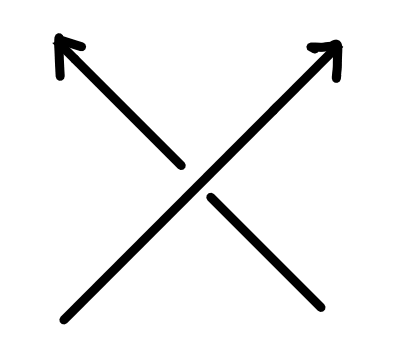
\includegraphics[width=1.5cm]{pic/lplus.png}} & $L_-$:\raisebox{-10pt}{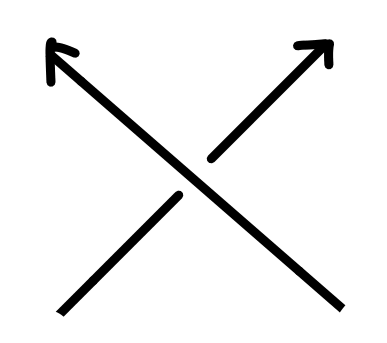
\includegraphics[width=1.5cm]{pic/lmin.png}} & $L_0$:\raisebox{-10pt}{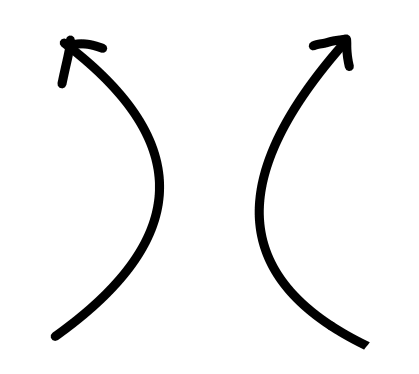
\includegraphics[width=1.5cm]{pic/l0.png}}
		\end{tabular}
	\end{center}

	\begin{block}{Skein Relation}
		In general, a skein relationship requires three link diagrams that are identical except at one crossing. To recursively define a knot (link) polynomial, a function $F$ is fixed and for any triple of diagrams and their polynomials labelled as above, \[F(L_+,L_-,L_0)=0.\]
	\end{block}

\end{frame}

\begin{frame}[c]
	\frametitle{Unlink}

	\begin{center}
		\begin{tabular}{ l  l l }
			$L_+$: \raisebox{-10pt}{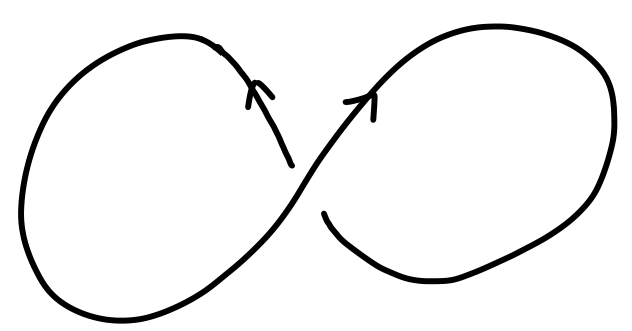
\includegraphics[width=2cm]{pic/unlinklp.png}} & $L_-$:\raisebox{-10pt}{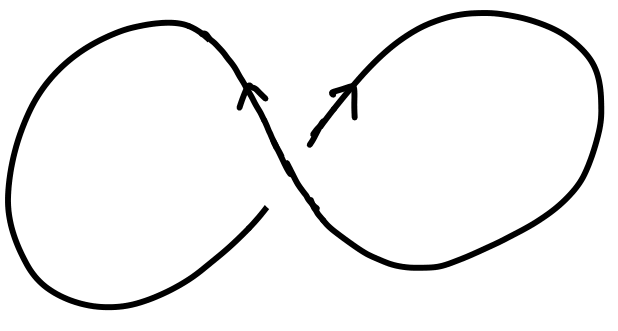
\includegraphics[width=2cm]{pic/unlinklm.png}} & $L_0$:\raisebox{-10pt}{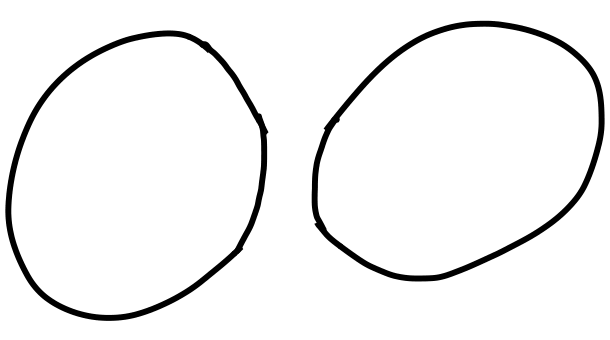
\includegraphics[width=2cm]{pic/unlinkl0.png}}
		\end{tabular}
	\end{center}
	\[t^{-1}V(L_+)- tV(L_-)+(t^{-1/2}-t^{1/2})V(L_0)=0\]
	But $L_+$ and $L_-$ are both the unknot, so $V(L_+)=V(L_-)=1$.
	\begin{align*}
		V(L_0) & =-\frac{t^{-1}- t}{t^{-1/2}-t^{1/2}} \\
		       & =-t^{-1/2}-t^{1/2}
	\end{align*}

\end{frame}

\begin{frame}[c]
	\frametitle{Yet Another Approach}
	% \begin{block}{Observation}
	% 	Given a knot diagram, if you change all $\KPB$ to either $\KPC$ or $\KPD$, then you arrive at an unlink.
	% \end{block}
	\begin{itemize}
		\item 	Label crossings in a knot diagram $D$ as $1,\dots,n$.
		\item A \emph{state} for $D$ is a function $s:\{1,\dots,n\}\to\{+1,-1\}$.
		\item There are $2^n$ states.
		\item Let $sD$ be the diagram by replacing each crossings according to \[\KPD \xleftarrow{\ \text{ if }s(i)=-1\ } \KPB \xrightarrow{\ \text{ if }s(i)=+1\ }  \KPC\]
		      for the $i^\text{th}$ crossing. Note that $sD$ is then an unlink.
		\item $|sD| =$ number of complements in the unlink $sD$.

	\end{itemize}
\end{frame}

\begin{frame}
	\frametitle{State Sum}
	\begin{block}{Definition-Theorem (Kauffman 1986)}
		Let $D$ be a link diagram (of an oriented link $L$) with $n$ crossings. Then the Kauffman bracket of $D$ is given by
		\[\langle D\rangle = \sum_s (A^{\sum_{i=1}^n s(i)} (-A^{-2}-A^2)^{|sD|-1}) \]
		where the summation is over all states $s:\{1,\dots,n\}\to\{+1,-1\}$.

		Therefore, the Jones polynomial of $L$ is given by
		\[V(L)= \left( (-A)^{-3w(D)}\langle \sum_s (A^{\sum_{i=1}^n s(i)} (-A^{-2}-A^2)^{|sD|-1}) \rangle \right)_{t^{1/2}=A^{-2}}.\]
	\end{block}
\end{frame}

\begin{frame}[c]
	\begin{figure}
		\centering
		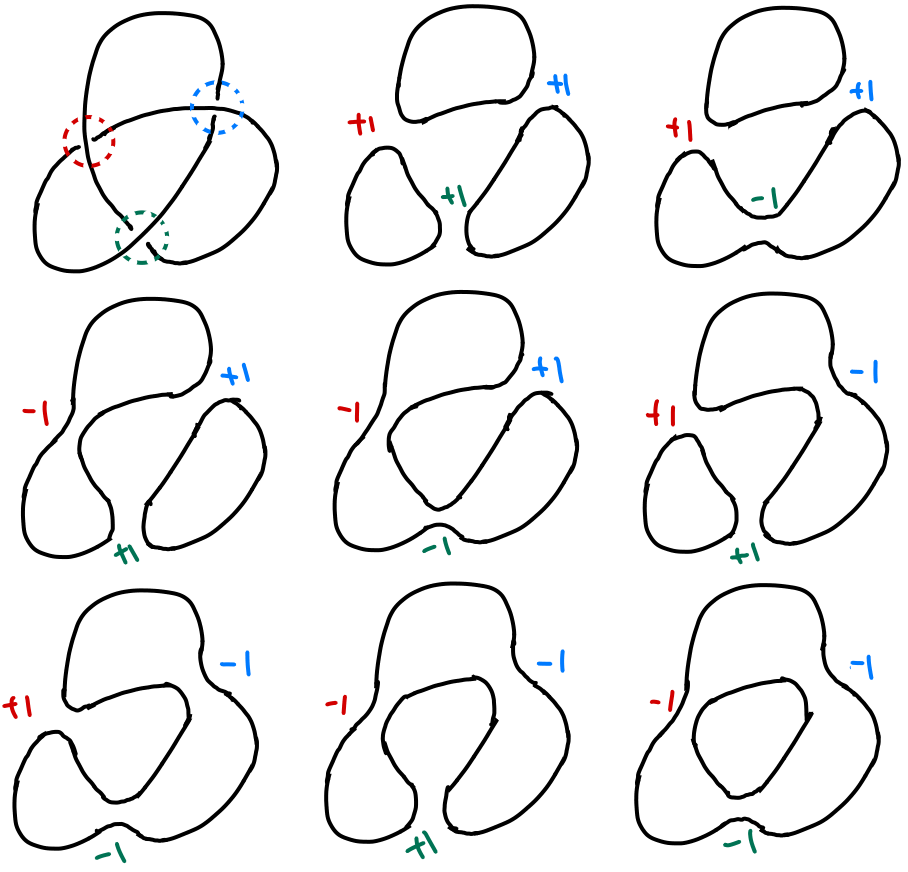
\includegraphics[width=6cm]{pic/statesum.png}
	\end{figure}
	\vspace{-0.4cm}
	\small
	\begin{align*}
		\hspace{-0.2cm}\langle\text{left-handed trefoil knot}\rangle & = 3A^{-1}+(A^{-3}+3A)(-A^{-2}-A^2)+A^3(-A^{-2}-A^{2})^2 \\
		                                                             & = A^7-A^3-A^{-5}
	\end{align*}

\end{frame}

\begin{frame}
	\frametitle{Open Problem}

	Facts:
	\begin{itemize}
		\item There are nontrivial knots $K_1\not=K_2$ with $V(K_1)=V(K_2)$.
		\item There are links with the same Jones polynomial as unlinks.
	\end{itemize}

	\begin{block}{Conjecture}
		The only knot with Jones polynomial $V(K)=1$ is the unknot.
	\end{block}

	The conjecture has been confirmed for several families of knots, including alternating knots and knots up to 23 crossings (as of 2019).
\end{frame}


\begin{frame}
	\frametitle{Coloured Jones Polynomials}

	None of the three methods discussed in this talk was Jones' original approach, where his formulation of the polynomial came from his study of operator algebras. His work is generalized to vast families of invariants, called quantum invariants.

	\begin{itemize}
		\item The coloured Jones polynomials is an infinite sequence of Laurent polynomials $\{J_{K,n}(t)\}_n$, encoding the Jones polynomial of $K$ and these of the links $K^s$ that are the \emph{parallels} of $K$.
		\item Formulae for $J_{K,n}(t)$ come from representation theory of $SU(2)$ by decomposition of tensor product of representations.
		\item $J_{K,n}(t)$ can be calculated from any knot diagram via processes such as skein theory, state sums, $R$-matrices, and ...
	\end{itemize}

\end{frame}

\begin{frame}
	\frametitle{Coloured Jones Polynomials}

	Fot this talk:

	\begin{itemize}
		\item  $J_{K,1}(t)=1$,
		\item  $J_{K,2}(t)=V(K)$ - original Jones polynomial,
		\item  $J_{K,3}(t)=V(K^2)-1$,
		\item  $J_{K,4}(t)=V(K^3)-2V(K)$,
		\item ...
	\end{itemize}
	\begin{figure}
		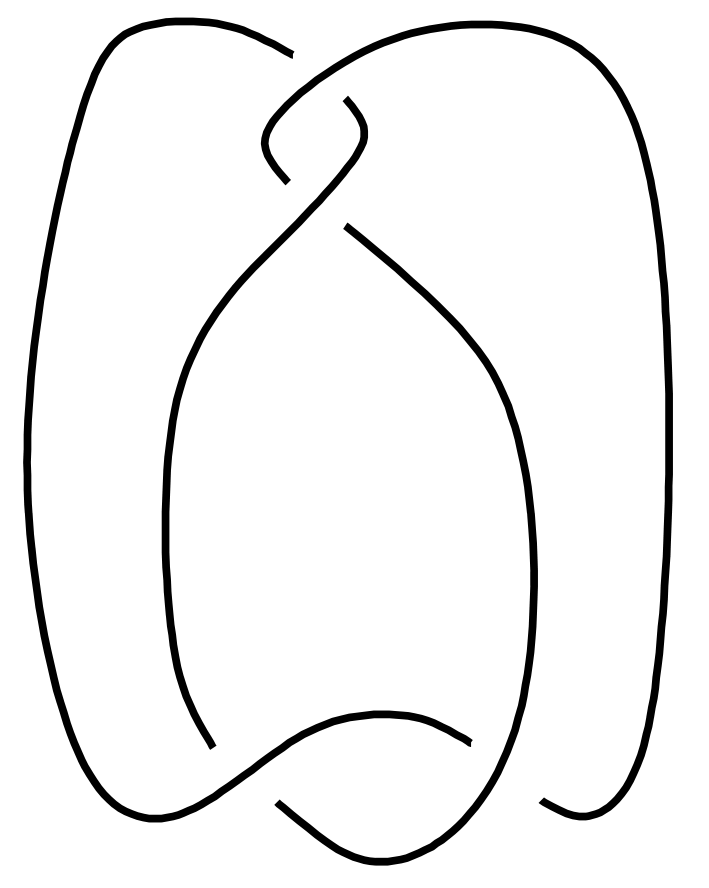
\includegraphics[width=2cm]{pic/fig8.png}
		\hspace{0.5cm}
		\includegraphics[width=2cm]{pic/fig83.png}
		\caption{Figure-8 knot and its parallels}
	\end{figure}

\end{frame}

\begin{frame}
	\frametitle{Conjecture}

	\begin{block}{Volume Conjecture}
		Let $K$ be a hyperbolic knot. Then \[\vol(K)=\lim_{N\to\infty}\frac{2\pi \log |\langle K\rangle_N |}{N},\] where \[\langle K\rangle_N=\lim_{q\to e^{2\pi i/N}} \frac{J_{K,N} (q)}{J_{\mbox{unknot},N}(q)}.\]
	\end{block}
	Note that this conjecture relates quantum invariants of knots to the hyperbolic geometry of knot complements.

\end{frame}

\end{document}